\documentclass[11pt]{article}

\usepackage{graphicx}
\usepackage[document]{ragged2e}
\usepackage{setspace}
\setlength\parindent{24pt}
\usepackage{indentfirst}
\usepackage{enumitem}
\usepackage{color}
\usepackage{hyperref}

\oddsidemargin 0mm
\evensidemargin 0mm
\textwidth 160mm
\textheight 200mm

\begin{document}
\begin{titlepage}
   \vspace*{\stretch{0.5}}
   \begin{center}
      \huge\textbf{JTAC - A JVM Alternative for Simple Java Programs}

      \bigskip
	  \small{\url{https://github.com/licarijd/java-arm-compiler}}

      \bigskip
      \Large CompSci 4TB3 - McMaster University, Department of Computing and Software

      \bigskip
      \bigskip
      \large \textit{Justin Licari - 001313781}

      \large \textit{Justin Staples - 001052815}

      \bigskip
      \bigskip
      \large April 20, 2018
   \end{center}
   \vspace*{\stretch{1.0}}

\end{titlepage}

\newpage

\tableofcontents

\thispagestyle{empty}

\newpage

\setcounter{page}{1}
\pagenumbering{arabic}

\section{Introduction}

\justifying
Compilers translate higher level code to lower level target code. Ultimately, for an executable program to run on a computer, high level code needs to be translated to a machine (assembly) language that can be understood by the computer hardware. Currently, one of the most common types of processors used for mobile devices is the ARM (Advanced RISC Machine) processor, which uses a reduced ISA (Patterson and Hennessy, n.d.). As well, one of the most popular types of processors used for personal computers is the Intel processor (x86 architecture), which uses a complex ISA (Wirth, 1996). 

\bigskip
This paper outlines JTAC (Java to ARM Compiler) - a tool that will be able to generate assembly code for a particular hardware platform (ARM, Intel, etc.), given source code in a high level language. We discuss our prototype, which is designed to transform Java code into ARM assembly code.

\bigskip
Java code is not typically compiled into an assembly language like ARM. The Java compiler actually translates the Java code into Java Bytecode, which is the instruction set understood by the Java Virtual Machine  (Sebesta, n.d). Therefore, to run a Java program, you must have the JVM installed on your computer. The motivation behind our project is to offer a different way of compiling and running a Java program (using ARM assembly instead of Bytecode). This will save developers the time and memory overhead of installing and running JVM.


\section{Technical Overview}

\subsection{Initialization File}

\justifying

JTAC is intended to be run on a UNIX based terminal, such as a Mac/Linux terminal, or even Cygwin on Windows. The initialization file is written in bash, and is a file input mechanism. {\tt JTAC.ini} starts the compilation process by:

\begin{enumerate}[label=\alph*)]
	\item taking a Java file as command line input: {\tt java\_file~=~\$1}
	\item passing it to the parser as a command line argument: {\tt python scanner.py \$1 }
\end{enumerate}

\subsection{Scanner}

The scanner will perform the first stage of lexical analysis. Source text (characters in the Java program file) will be classified as symbols, and converted to a sequence of symbols).

\bigskip
A high-level description of this program’s methods and their functionality:

\bigskip
\textbf{\tt main():}

\begin{enumerate}[label=\alph*)]
	\item Removes comments from input. 
	\item Group source text into words based on whitespace, and construct a list of words.
	\item Remove whitespace.
	\item Call getSym() on the first word in the list.
\end{enumerate}

\textbf{\tt getSym():}

\begin{enumerate}[label=\alph*)]
	\item First check if all of the words in the list have been checked. If words still need to be checked, check for reserved words by calling {\tt checkForReservedWords()}, then check for reserved symbols by calling {\tt checkForReservedSymbols()}. 

	\item If all words have been checked, add the `eof' symbol and terminate the program successfully.
	\item Recursively call getSym() until all words have been checked.
\end{enumerate}

\textbf{\tt checkForReservedWords():}

\begin{enumerate}[label=\alph*)]
	\item First, check if the word is a number.
	\item If not, check if the word can be classified as a reserved reserved symbol, such as {\tt public}, {\tt class}, {\tt main}, etc.
\end{enumerate}

\textbf{\tt checkForReservedSymbols():}

\begin{enumerate}[label=\alph*)]
	\item Check if the word is a 2-digit relational operator, such as `==' by calling {\tt checkRelationalOp()}.
	\item Check for reserved symbols, such as `=', `+', `-', etc.
	\item If none can be found, assume the word is an identifier.
\end{enumerate}

\textbf{\tt checkForNum():}

\begin{enumerate}[label=\alph*)]
	\item Checks if the current word is a number using {\tt type(sym) == int}
\end{enumerate}

Now, a low-level explanation of this program’s functionality is given in the following sections.

\bigskip
\textbf{Imports:}

\bigskip
The {\tt sys} library is imported to allow the program to take command-line arguments.

\bigskip
\textbf{Global Variables:}

\bigskip
A list of words are generated according to whitespace. A variable, {\tt currentPosition}, represents the position of a word in this list. When each character in a word is being checked individually, {\tt currentBlockPosition} represents the position of a character in a word.

\subsubsection{{\tt main()}}

The input file is read and split into a list.

~
\begin{center}

\includegraphics[scale=0.6]{1}
\end{center}
~

Comments and whitespace are removed.

~
\begin{center}
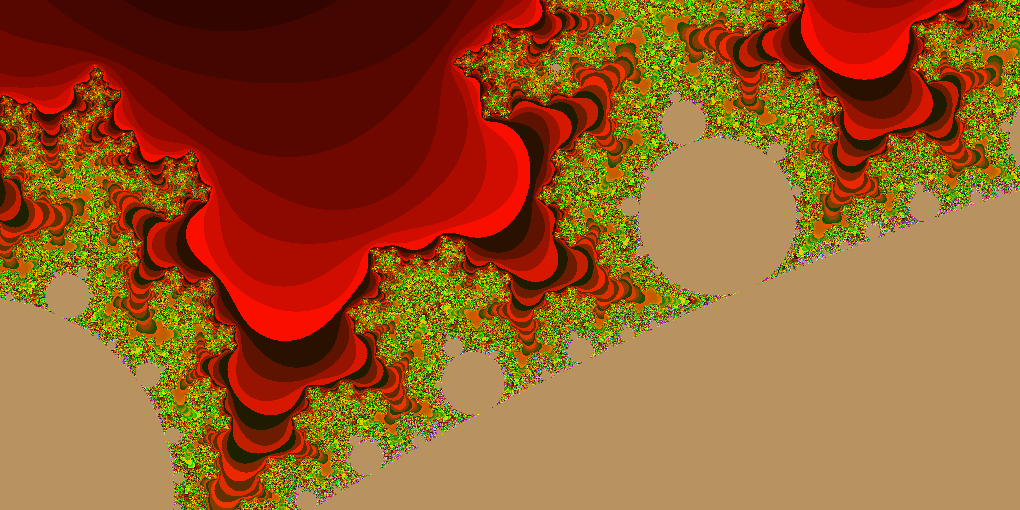
\includegraphics[scale=0.6]{2}
\end{center}
~

{\tt getSym()} is called.

~
\begin{center}

\includegraphics[scale=0.6]{3}
\end{center}
~

\subsubsection{{\tt getSym()}}

First, check for reserved words.

~
\begin{center}

\includegraphics[scale=0.6]{4}
\end{center}
~

If the entire word isn't reserved, check individual characters.

~
\begin{center}

\includegraphics[scale=0.6]{5}
\end{center}
~

Call getSym() on the next word.

~
\begin{center}

\includegraphics[scale=0.6]{3}
\end{center}
~

Once all words have been checked, end the program.

~
\begin{center}

\includegraphics[scale=0.6]{6}
\end{center}
~

\subsubsection{{\tt checkForReservedWords()}}

{\tt sym}, which represents the current word, and {\tt words}, which represents the list of words are passed as arguments. {\tt currentBlockPosition} is set to 0 to indicate that a new block of characters are being checked, and {\tt checkForNum()} is called.

~
\begin{center}

\includegraphics[scale=0.6]{7}
\end{center}
~

Then, the current symbol is checked against reserved words in Java.

~
\begin{center}

\includegraphics[scale=0.6]{8}
\end{center}
~

If the word isn’t a reserved word in Java, check if it is comprised of reserved symbols.

~
\begin{center}

\includegraphics[scale=0.6]{9}
\end{center}
~

If the word isn’t a reserved word in Java and is not comprised of reserved symbols, assume it is an identifier.

~
\begin{center}
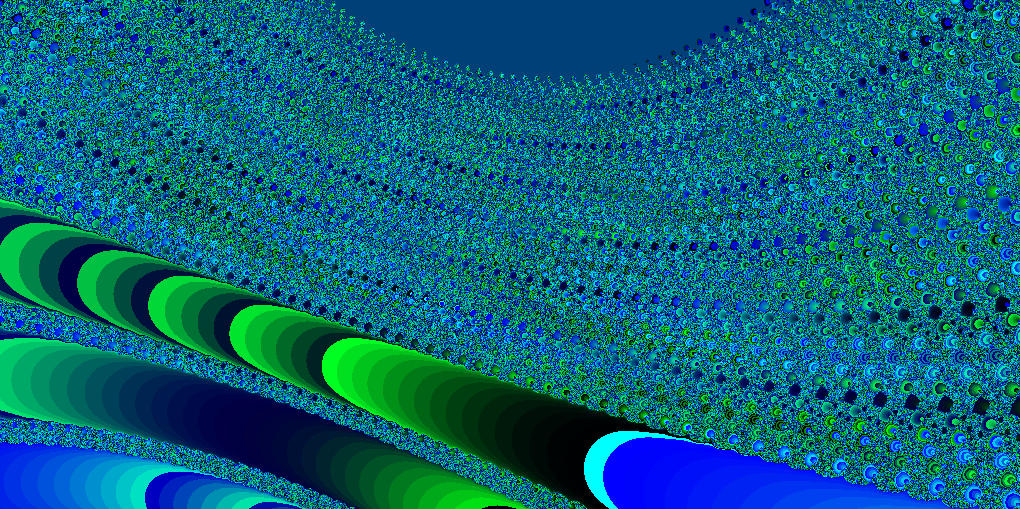
\includegraphics[scale=0.6]{10}
\end{center}
~

\subsubsection{{\tt checkForReservedSymbols()}}

{\tt sym}, which represents the current word, and {\tt words}, which represents the list of words are passed as arguments.

~
\begin{center}
\includegraphics[scale=0.6]{11}
\end{center}
~

If the symbol is a reserved relational operator, the word may be a 2-digit relational operator. {\tt checkRelationalOp()} is run to check this.

~
\begin{center}
\includegraphics[scale=0.6]{12}
\end{center}
~

Next, single digit reserved characters are checked.

~
\begin{center}
\includegraphics[scale=0.6]{13}
\end{center}
~

\subsubsection{{\tt checkForNum()}}

{\tt sym}, which represents the current word, is passed as an argument. The symbol is categorized as a number if it is an integer.

~
\begin{center}
\includegraphics[scale=0.6]{14}
\end{center}
~

\subsubsection{{\tt checkRelationalOp()}}

{\tt Sym}, which represents the current word, is passed as an argument. A reference is also made to the next symbol, and both the current symbol and next symbol are checked to determine if a 2-digit relational operator is present.

~
\begin{center}
\includegraphics[scale=0.6]{15}
\end{center}
~

~
\begin{center}
\includegraphics[scale=0.6]{16}
\end{center}
~

\subsection{A Simple Grammar for Java Programs}

Shown below is a Java grammar for simple Java programs consisting of only a main method and print statements which prints a String. Terminals are shown in lower case and non-terminals are shown in upper-case:

$$ PROG \rightarrow (IMPORT\_DECLARATION)^{*} ~ CLASS\_DECLARATION$$
$$ IMPORT\_DECLARATION \rightarrow "import" ~["static"] ~identifier ~";" $$
$$ CLASS\_DECLARATION \rightarrow "public~class" ~ identifier~"\{" MAIN\_METHOD\_DECLARATION~"\}" $$
$$ MAIN\_METHOD\_DECLARATION \rightarrow "public~static~void~main~(String~[]~args) \{"~METHOD\_BODY~"\}" $$
$$ METHOD\_BODY \rightarrow PRINT\_STATEMENT ~ \mid ~ EXIT\_STATEMENT$$
$$ PRINT\_STATEMENT \rightarrow "System.out.println(" ~identifier~");" $$
$$ EXIT\_STATEMENT \rightarrow "System.exit(0);" $$
$$ identifier \rightarrow [a-zA-Z]+ $$

\subsection{Parser}

The goal of the recursive descent parser is to construct a syntax tree for the sentence generated from {\tt scanner.py}, get the context info for the syntax tree, and accept/reject the sentence. 

The start symbol, PROG, is implemented with the prog() method, which checks for imports and class declaration (these are found at the top of Java programs). 

~
\begin{center}
\includegraphics[scale=0.6]{17}
\end{center}
~

{\tt main()} takes a sentence generated from {\tt scanner.py} as a command-line argument, and starts {\tt prog()} to begin the recursive descent process.

~
\begin{center}
\includegraphics[scale=0.6]{18}
\end{center}
~

For each production, methods are called in the order that their corresponding non-terminal symbol appears. Sentences are accepted or rejected based on an expected set of terminal symbols, or an unexpected terminal symbol. After a terminal symbol is checked, the program iterates to the next symbol. This code illustrates the process for the CLASS\_DECLARATION production. 

~
\begin{center}
\includegraphics[scale=0.6]{19}
\end{center}
~

This code illustrates the same process for the MAIN\_METHOD\_DELCARATION production.

~
\begin{center}
\includegraphics[scale=0.6]{20}
\end{center}
~

\subsection{Code Generator}

\justifying
As mentioned before, Java programs are typically compiled into byte code which is then interpreted on the JVM (Java Virtual Machine). JTAC bypasses this requirement by generating ARM code that can be run on any ARM processor or ARM virtual machine. 

\bigskip
It was necessary to understand the subset of the ARM instruction set that was necessary for the scope of the project. Meaning, it was necessary to identify which instructions needed to have code generated. Because of the need to load constants and variables, the {\tt MOV} (move) and {\tt LDR} (load register) instructions are required. As well, to actually execute print statements and to exit the program, the {\tt SWI} (software interrupt) instruction is needed. This instruction hands control over to the operating system and performs a certain function depending on which flags are set. 

\bigskip
The code generator module for JTAC follows the design pattern of the one studied in the class. The module serves as a small library of routines that are responsible for generating code for individual parts of the program. The module keeps tracks of the 16 available all purpose registers in the ARM architecture by use Python dictionaries. Similar to the pattern used by the compiler for P0, the methods in the code generator module are called at the appropriate time while the parsing procedures are taking place. The following sections outline the details of some of the these methods. 

\subsubsection{{\tt genProgEntry()}}

This method is called at the very beginning of the parsing procedures. It sets up necessary labels for the program entry point, which is the {\tt main()} method. As well, it creates a label for the data section, which is where string variables will be stored. 

\bigskip
This procedure will also automatically write two instructions to the output. These two {\tt MOV} instructions fill registers R0 and R7 with appropriate values so that the operating system will issue a print command the next time that a software interrupt is called. Due to the simple structure of the Java grammar proposed, it can be certain that the first type of statement encountered will be a print statement. So, these flags are set as part of the set up routine. 

\subsubsection{{\tt genPrintStatement()}} 

This routine is responsible for generating ARM code for Java print statements. Each print statement requires a few different instructions. First, the size of the string is moved into a register with the {\tt MOV} command. Next, because the string is stored in memory, its address is moved into register using the {\tt LDR} instruction. With these two values loaded in, the system call to print the string can be performed. This is done using {\tt SWI}. It will print the number of bytes specified in register R2 starting from the address stored in R1. 

\bigskip
Once the instructions are generated, the values of the registers are updated. Lastly, for each new print statement, the data section of the ARM code is updated to allocate space for each new string.

\subsubsection{{\tt genProgExit()}}

When the parser detects that there is a system exit statement, it knows that there must be no more print statements and that the program is terminating. In preparation of the program exit, the R7 register is set to a different value than before. This will serve as a flag that tells the operating system that the next time there is a software interrupt to exit, instead of printing or doing something else. The routine is simple, it just sets the flag and then writes the {\tt SWI} instruction to exit. 

\subsubsection{\tt genProgram()}

If the parsing procedure completes succesfully, then this method will take the code generated for the main method and the code generated for the data section and append them together. This creates one output, which is then written to a file. 

\section{Discussion}

\justifying

The JTAC prototype is able to compile simple Java programs consisting of the following elements:

\begin{enumerate}[label=\alph*)]
	\item main method
	\item print statements
	\item exit statements
\end{enumerate}

However, JTAC can easily be extended to include:

\begin{enumerate}[label=\alph*)]
	\item variable declaration and assignment
	\item arithmetic
	\item defined methods
\end{enumerate}

Here, we discuss code modifications to the various components of JTAC to make these extensions.

\subsection{{\tt scanner.py}}

\subsubsection{Arithmetic}

{\tt checkForReservedSymbols(symList,words)} already contains conditionals which recognize arithmetic operators.

~
\begin{center}
\includegraphics[scale=0.6]{21}
\end{center}
~

\subsubsection{Variable declaration and assignment}

{\tt checkForReservedSymbols(symList,words)} would need to be extended to recognize data types, such as {\tt int} and {\tt String}.

~
\begin{center}
\includegraphics[scale=0.6]{22}
\end{center}
~

\subsubsection{Methods}

Most words needed to declare methods are already recognized in {\tt checkForReservedSymbols(symList,words)}. Certain symbols, such as {\tt void}, would need to be added.

~
\begin{center}
\includegraphics[scale=0.6]{23}
\end{center}
~

\subsection{Java Grammar}

The following productions, highlighted in blue, would need to be added to define variable declaration and assignment (Strings and integers are shown as an example), arithmetic expressions, and method definition.

{\scriptsize 
$$ PROG \rightarrow (IMPORT\_DECLARATION)^{*} ~ CLASS\_DECLARATION$$
$$ IMPORT\_DECLARATION \rightarrow "import" ~["static"] ~identifier ~";" $$
$$ CLASS\_DECLARATION \rightarrow "public~class" ~ identifier~"\{"METHOD\_DECLARATION^{*} ~ MAIN\_METHOD\_DECLARATION~"\}" $$
{\color{blue} $$ METHOD\_DECLARATION \rightarrow TYPE ~ identifier ~ "(" ~ (TYPE ~ identifier)^{*} ~")" ~ METHOD\_BODY ~ "\}" $$}
$$ MAIN\_METHOD\_DECLARATION \rightarrow "public~static~void~main~(String~[]~args) \{"~METHOD\_BODY~"\}" $$
$$ METHOD\_BODY \rightarrow PRINT\_STATEMENT ~ \mid ~ EXIT\_STATEMENT ~ \mid ~ {\color{blue} ARITHMETIC\_STATEMENT ~ \mid ~ ASSIGNMENT}$$
$$ PRINT\_STATEMENT \rightarrow "System.out.println(" ~identifier~");" $$
$$ EXIT\_STATEMENT \rightarrow "System.exit(0);" $$
{\color{blue} $$ ARITHMETIC\_STATEMENT \rightarrow (identifier ~ ARITHMETIC\_OP)^{+} identifier $$ 
$$ ARITHMETIC\_OP \rightarrow "+" ~\mid~ "-" ~\mid~ "/" ~\mid~ "*" $$}
{\color{blue} $$ TYPE \rightarrow "boolean" ~\mid~ "int" ~\mid~ "String" $$
$$ STRING \rightarrow \\" . \\"  $$ 
$$ INT \rightarrow [0-9]+ $$}
$$ identifier \rightarrow [a-zA-Z]+ $$
}

\subsection{{\tt rdparser.py}}

New methods would need to be created to handle variable declaration and assignment (Strings and integers are shown as an example), arithmetic expressions, and method definition, as defined in the grammar above. For example, the following code could be used to accept or reject a method body.

~
\begin{center}
\includegraphics[scale=0.6]{24}
\end{center}
~

It should be noted that the above code includes a conditional branch to handle arithmetic (only for integers in this example).

~
\begin{center}
\includegraphics[scale=0.6]{25}
\end{center}
~

\subsection{{\tt generator.py}}

The code generator could be extended in a similar way to handle these new features. New methods could be added to this module that could be responsible for generating code for arithmetic operations or assignment statements. Consider the following statement, {\tt x = y + z}, which adds two integers. A method in the code generator might generate the following instructions.

~
\begin{center}
\includegraphics[scale=0.6]{26}
\end{center}
~

Here, the values of y and z have been loaded in from memory. Their sum is stored in the register R3, and then that result is written to the memory address of x. 

As well, extending this code generator to handle method calls can be done in a very similar way to how it is done in the P0 compiler. Namely, when a procedure is entered or exited, there are instructions generated for keeping track of the stack pointer. This can be done the same way for Java methods.

As we might have expected, the JTAC solution for compiling Java code has shown significantly faster compile times. One experiment that was done was to compile a simple HelloWorld Java program using two different approaches. The first was to compile it using a common IDE (Intelli-J) and the other was to compile it using JTAC. The following figures summarize the compile times for each method.

~
\begin{figure}[h]
\centering
\includegraphics[scale=0.35]{28}
\caption{Compile time in Intelli-J was 2.491 seconds.}
\end{figure}
~

~
\begin{figure}[h]
\centering
\includegraphics[scale=1]{29}
\caption{Compile time in JTAC was 0.207 seconds.}
\end{figure}
~

~
\begin{figure}[h]
\centering
\includegraphics[scale=0.35]{27}
\caption{A side by side comparison of the compiler times.}
\end{figure}
~

Another important consideration for developers is the memory requirement to set up and run their programs. JTAC offers a solution that is significantly more lightweight than an IDE solution. The following figure summarizes the memory expense for each option. Clearly, JTAC offers significant improvements.

~
\begin{center}
\includegraphics[scale=0.30]{30}
\end{center}
~

\section{Conclusion}

JTAC is a program that accepts a potential Java program as input. JTAC performs lexical and syntactic analysis, and generates the relevant ARM code once a valid Java program is detected. In theory, this ARM code could then be run on a computer that has an ARM processor or that has access to an ARM virtual environment.

\bigskip
As expected, JTAC is significantly smaller and faster than JVM for simple Java programs. JTAC is 26 kilobytes as opposed to 775 megabytes to run program using JRE, JDK, and IntelliJ, and can compile a simple HelloWorld program in 0.207s as opposed to 2.491s through Intelli-J.

\bigskip
We discussed how to extend our code to handle arithmetic, variable declaration and assignment, and methods. To extend JTAC further (for example, to handle interfaces), developers would first have to extend the scanner to recognize new reserved words, such as {\tt static} in {\tt checkForReservedWord()s}, and new symbols, such as the mod symbol, \%, in {\tt checkForReservedSymbols()}. New productions would need to be added to JTAC’s Java grammar, (e.g INTERFACE\_DECLARATION $\rightarrow$ ...) and the appropriate productions would need to be added as new methods (e.g def interface\_declaration(sentence)) in rdparser.py. Existing productions, such as PRINT\_STATEMENT, would need to be extended to handle more complex arguments. Finally, additional code generation methods would need to be added in {\\tt generator.py}.

\newpage
\newpage

\section*{References}

[1] Anon, (2018). [ebook] Available at: http://vision.gel.ulaval.ca/~jflalonde/cours/1001/h17/docs/arm-instructionset.pdf [Accessed 21 Apr. 2018].

\bigskip
[2] Ltd., A. (2018). Architecture | Instruction Sets – Arm Developer. [online] ARM Developer. Available at: https://developer.arm.com/products/architecture/instruction-sets [Accessed 21 Apr. 2018].

\bigskip
[3] Patterson, D. and Hennessy, J. (n.d.). Computer Organization and Design.

\bigskip
[4] Sebesta, R. (n.d.). Concepts of Programming Languages.

\bigskip
[5] Wirth, N. (1996). Compiler Construction. Amsterdam: Addison-Wesley.


\end{document}